% Copyright 2003--2007 by Till Tantau
% Copyright 2010 by Vedran Mileti\'c
%
% This file may be distributed and/or modified
%
% 1. under the LaTeX Project Public License and/or
% 2. under the GNU Free Documentation License.
%
% See the file doc/licenses/LICENSE for more details.

% $Header: /Users/joseph/Documents/LaTeX/beamer/doc/themeexamples/beamerthemeexample.tex,v 5a25f58600c3 2010/04/27 12:17:50 rivanvx $


\documentclass[aspectratio=169,1pt]{beamer}

\usetheme{RomaTorVergata}

\beamertemplatetransparentcovered	%multi step visibili ma in non evidenziati
%remove beamer navigation links
%\beamertemplatenavigationsymbolsempty
\setbeamertemplate{navigation symbols}{}
\usepackage{times}
\usepackage[T1]{fontenc}
\usepackage[export]{adjustbox}	%figure align extra keys
\usepackage{graphicx}
\graphicspath{ {../imgs/} } % imgs searched from this dir
%%bold in verbatim
%\usepackage{fancyvrb}
%\newcommand\verbBoldize[1]{\textbf{#1}}
%\usepackage{tgcursor}

\newcommand{\backupbegin}{
   \newcounter{framenumberappendix}
   \setcounter{framenumberappendix}{\value{framenumber}}
}
\newcommand{\backupend}{
   \addtocounter{framenumberappendix}{-\value{framenumber}}
   \addtocounter{framenumber}{\value{framenumberappendix}} 
}
%
%%%%%%%%%%%%%%%%%%%%%%%%%%%%%%%%%% CODE EMBEDD %%%%%%%%%%%%%%%%%%%%%%%%%%%%%%%%%
\usepackage{listings,color,tcolorbox} 
\definecolor{myDarkBlue}{rgb}{0,0.0,.78}      
%CONFIG CODE LISTINGS
\definecolor{mygreen}{rgb}{0,0.6,0}      
\definecolor{mygray}{rgb}{0.5,0.5,0.5}   
\definecolor{mymauve}{rgb}{0.58,0,0.82}  
\definecolor{background}{RGB}{255, 255, 255}

\makeatletter
\newcommand{\srcsize}		{\ttfamily\@setfontsize{\srcsize}{5.5pt}{6pt}}
\newcommand{\srcsizeNums}	{\@setfontsize{\srcsize}{2.5pt}{2.5pt}}
\makeatother

\lstloadlanguages{C}
\lstdefinestyle{C_typedefs}{
	language=C,
	keywordstyle=\color{red},
	%morecomment=[l][\color{purple}]{\#pragma}	 %TODO FIX
	morekeywords={inline,uint,ulong,ushort,idx_t,spmat,CONFIG},
	morecomment=[l][\color{mygreen}]{\#},	 %TODO FIX
	%keywordstyle=\color{mygreen},
	%classoffset=2,
	%morekeywords=[\color{mygreen}]{CAT}
}
\lstset{ 
  %escapechar=\%,                  %%EMBEDD LATEX CODE IN SOURCE CODE 
  escapeinside={*@}{@*},       %%EMBEDD LATEX CODE IN SOURCE PARTI RACCHIUSE DA QUESTE DUE COPPIE              
  %captionpos=b,                    % sets the caption-position to bottom 
  tabsize=2,                       % sets default tabsize to 2 spaces 
  %title=\lstname                   % show the filename of files included with \lstinputlisting; also try caption instead of title 
  linewidth=\textwidth,
  %basicstyle=\tiny,        % the size of the fonts that are used for the code 
  basicstyle= {\ttfamily\srcsize},
  numberstyle={\ttfamily\srcsizeNums},
  stepnumber=1,                    % the step between two line-numbers. If it's 1, each line will be numbered 
  numbersep=1pt,                   % how far the line-numbers are from the code 
  %basewidth=0.6em,   fontadjust=true, %fontSizes config in manual 
  %TODO NOT WORK xleftmargin=\dimexpr-\csname @totalleftmargin\endcsname]
  numbers=left,                    % where to put the line-numbers; possible values are (none, left, right) 
  numberfirstline=true,   firstnumber=1, 
  %frame=lines,                   % bordo attorno al codice 
  %keepspaces=true,                 % keeps spaces in text, useful for keeping indentation of code (possibly needs columns=flexible) 
  %keywordstyle=\color{red},       % keyword style 
  language=C, style=C_typedefs, 
  %deletekeywords={...},            % if you want to delete keywords from the given language 
  %rulecolor=\color{black},         % if not set, the frame-color may be changed on line-breaks within not-black text (e.g. comments (green here)) 
  %showspaces=false,                % show spaces everywhere adding particular underscores; it overrides 'showstringspaces' 
  showstringspaces=false,          % underline spaces within strings only 
  %showtabs=false,                  % show tabs within strings adding particular underscores 
  backgroundcolor=\color{background},   % choose the background color; you must add \usepackage{color} or \usepackage{xcolor}; should come as last argument 
  breakatwhitespace=false,         % sets if automatic breaks should only happen at whitespace 
  %breaklines=true,                 % sets automatic line breaking 
  commentstyle=\color{mygreen},    % comment style 
  extendedchars=false,             % lets you use non-ASCII characters; for 8-bits encodings only, does not work with UTF-8 
  stringstyle=\color{mymauve},     % string literal style 
} 
%\lstset{
%  %escapechar=\%,                  %%EMBEDD LATEX CODE IN SOURCE CODE
%  escapeinside={*@}{@*},       %%EMBEDD LATEX CODE IN SOURCE PARTI RACCHIUSE DA QUESTE DUE COPPIE             
%  captionpos=b,                    % sets the caption-position to bottom
%  tabsize=2,                       % sets default tabsize to 2 spaces
%  %title=\lstname                   % show the filename of files included with \lstinputlisting; also try caption instead of title
%  basicstyle=\footnotesize,        % the size of the fonts that are used for the code
%  basewidth=0.6em,   fontadjust=true, %fontSizes config in manual
%  numberstyle=\tiny, % the style that is used for the line-numbers
%  numbersep=3pt,                   % how far the line-numbers are from the code
%  numbers=left,                    % where to put the line-numbers; possible values are (none, left, right)
%  numberfirstline=true,   firstnumber=1,
%  stepnumber=1,                    % the step between two line-numbers. If it's 1, each line will be numbered
%  frame=lines,                   % bordo attorno al codice
%  keepspaces=true,                 % keeps spaces in text, useful for keeping indentation of code (possibly needs columns=flexible)
%  keywordstyle=\color{red},       % keyword style
%  language=C,             % the language of the code
%  style=C_typedefs,
%  morekeywords={uint,ulong}        % add more keywords to the set
%  %deletekeywords={...},            % if you want to delete keywords from the given language
%  rulecolor=\color{black},         % if not set, the frame-color may be changed on line-breaks within not-black text (e.g. comments (green here))
%  showspaces=false,                % show spaces everywhere adding particular underscores; it overrides 'showstringspaces'
%  showstringspaces=false,          % underline spaces within strings only
%  showtabs=false,                  % show tabs within strings adding particular underscores
%  backgroundcolor=\color{white},   % choose the background color; you must add \usepackage{color} or \usepackage{xcolor}; should come as last argument
%  breakatwhitespace=false,         % sets if automatic breaks should only happen at whitespace
%  breaklines=true,                 % sets automatic line breaking
%  commentstyle=\color{mygreen},    % comment style
%  extendedchars=false,             % lets you use non-ASCII characters; for 8-bits encodings only, does not work with UTF-8
%  stringstyle=\color{mymauve},     % string literal style
%}
%%%%%%%%%%%%%%%%%%%%%%%%%%%%%%%%%%%%%%%%%%%%%%%%%%%%%%%%%%%%%%%%%%%%%%%%%%%%%%%%

%\usefonttheme[onlylarge]{structurebold}
%\setbeamerfont*{frametitle}{size=\smallsize,series=\bfseries}
% Add option [numbering=none] to disable the footer progress bar
% Add option [numbering=fullbar] to show the footer progress bar as always full with a slide count

%%%SET SMALL CAPTION SIZE
%\setbeamerfont{caption}{size=\tiny}
%\usepackage[font=small, justification=centering]{caption}
%\DeclareCaptionFont{tiny}{\tiny}
%\captionsetup{font=tiny}
%\setbeamercolor{caption name}{fg=black}

%%custom beamer title
%\setbeamertemplate{frametitle}{%
%    \nointerlineskip%
%    \begin{beamercolorbox}[wd=\paperwidth,ht=1.0ex,dp=0.1ex]{frametitle}
%        \hspace*{1ex}\insertframetitle%
%    \end{beamercolorbox}%
%}

%------------------------------------------------

\title{Sp3MM for AMG}
\subtitle{Sparse Triple Matrix Matrix Multiplication\\for\\AlgebraicMultiGrid}

\author{Andrea Di Iorio}
\institute{Università di Roma Tor Vergata}
\date{22/04/2022}

%COMMANDS - MACROS

\newcommand{\vvv}[1]{{\small\texttt{#1}}}
\newcommand{\voidLine}{\par\null\par\noindent}
\newcommand{\paragraphh}[1]{\paragraph{#1}\mbox{}\\}
\newcommand{\citebf}[1]{\textbf{\cite{#1}}}
\newcommand{\refbf}[1]{\textbf{\ref{#1}}}
\newcommand{\nnz}	{non zero }
\newcommand{\nnnz}	{numero di non zeri }
\newcommand{\rowbyrow}	{row-by-row }
\newcommand{\amgforpsblas}	{\url{https://github.com/sfilippone/amg4psblas}}


%\AtBeginSubsection[]{%
%  \frame<beamer>{ 
%    \frametitle{title}   
%    \tableofcontents[currentsection,currentsubsection] 
%  }
%}

%chapter introduction slide (simple)
\AtBeginSection[]{
  \begin{frame}<beamer>[noframenumbering]
  \vfill
  \centering
  \begin{beamercolorbox}[sep=8pt,center,shadow=true,rounded=true]{title}
    \usebeamerfont{title}\insertsectionhead\par%
  \end{beamercolorbox}
  \tableofcontents[currentsection,currentsubsection] 
  \vfill
  \end{frame}
}

\begin{document}

\newcommand\blfootnote[1]{%
  \begingroup
  \renewcommand\thefootnote{}\footnote{{\tiny #1 }}%
  \addtocounter{footnote}{-1}%
  \endgroup
}

%%%%%%%%%%%%%%%%%%%%%%  TITLE PAGE  %%%%%%%%%%%%%%%%%%%%%%%%%%%%%%%%%%%%%%%%%%%%
%\begin{frame}
%	%%automatiche from prof theme...
%	%\titlepage
%	%Studente: Andrea Di Iorio	Relatore: Salvatore Filippone
%	%manual cover page
%	\begin{center}
%	\par\noindent\rule{\textwidth}{0.4pt}	%\HRule 
%	\vspace{.7cm}
%	{\Large \bfseries Sparse Triple Matrix Matrix Multiplication\\for\\AlgebraicMultiGrid}
%	\vspace{.7cm}
%	\par\noindent\rule{\textwidth}{0.4pt}	%\HRule 
%	\end{center}
%	\vfill \vspace{0.5cm}
%	\begin{minipage}[t]{0.4\textwidth}
%	\begin{flushleft} \large
%	\emph{Relatore: Salvatore Filippone}\\
%	\end{flushleft}
%	\end{minipage}
%	
%	\begin{minipage}[t]{0.4\textwidth}
%	\begin{flushright} \large
%	\emph{Studente:  Andrea Di Iorio\\Matricola: 0277550}\\
%	\end{flushright}
%	\end{minipage}
%\end{frame}

\begin{frame}

\includegraphics[width=\linewidth,keepaspectratio]{titlePageFull_InProgress.svg.pdf}
\end{frame}
%%%%%%%%%%%%%%%%%%%%%%  TITLE PAGE  %%%%%%%%%%%%%%%%%%%%%%%%%%%%%%%%%%%%%%%%%%%%
\begin{frame}<beamer>[noframenumbering]{Outline}
	\tableofcontents
\end{frame}

\section{Introduzione}
\begin{frame}	{Problema Affrontato}
\begin{itemize}
	\item	Progettare e realizzare implementazioni parallele mediante \emph{openMP} \\
			del triplo prodotto tra matrici sparse (\emph{Sp3MM})
	\pause
	\item	Necessarie nella fase di setup dei metodi Algebraic Multi Grid (\emph{AMG})
	\begin{itemize}
		\item	in combinazione di solutori iterativi di sistemi di sistemi lineari sparsi $Ax=b$
		\pause
		\item	Prodotto di Galerkin:\\
			$A_{l+1} = (P_l)^T \cdot A_l \cdot P_l  \quad \text{dove:} ~
			\begin{aligned}  
				& A \in \mathbb{R}^{n \times n} \\  
				& A_0 = A\\  
				& A_{l+1}  \in \mathbb{R}^{n_{l+1} \times n_{l+1}} \quad \text{con}~ n_{l+1}<n \end{aligned} $%\right\}$%~l=0,\dots,nl-1
	\end{itemize}
\end{itemize}
\voidLine
\centering
\includegraphics[width=.33\linewidth,keepaspectratio]{Multigrid_Visualization_wikipedia.png}
%Semplice intro,  un contesto applicativo segue
%(FDM) are a class of numerical techniques for solving differential equations by approximating derivatives with finite differences. Both the spatial domain and time interval (if applicable) are discretized, or broken into a finite number of steps, and the value of the solution at these discrete points is approximated by solving algebraic equations containing finite differences and values from nearby points. 

\end{frame}

\section{Algoritmi Esistenti}
\begin{frame} {Formulazioni SpMM}
Considerando la moltiplicazione tra matrici sparse $C = A\cdot B$
\voidLine
\centering
$
\begin{aligned}
  &\text{Inner-product}	&& \qquad c_{ij} = \sum\limits_{k \in I_i(A) \cap I^j(B) }  a_{ik} \ast  b_{kj}   \\
  &\text{Row-by-row}	&& \qquad c_{i*} = \sum\limits_{k \in I_i(A)}  a_{ik} \ast  b_{k*}  \\
  &\text{Col-by-col}	&& \qquad c_{*j} = \sum\limits_{k \in I^j(B)}  a_{*k} \ast  b_{kj}   \\
  &\text{Outer-product}	&& \qquad C = \sum\limits_{i=1}^k  a_{*i} \otimes  b_{i*}                \\
\end{aligned}
$\\
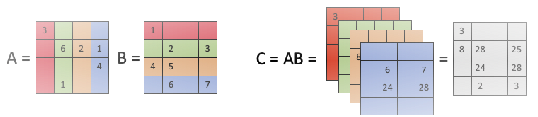
\includegraphics[width=.33\linewidth,keepaspectratio]{outerProductExampleVisual_ESC.png}

\blfootnote{Gao, Jianhua \& Ji, Weixing \& Tan, Zhaonian \& Zhao, Yueyan
«A Systematic Survey of General Sparse Matrix-Matrix Multiplication»}
%Notazione:
%I_I: indici di rigai, I^j indici di colonna j, I(i,j): indici di elementi non zero riga e col
%Outer product: somma di matrici a rango 1 generate dal Prodotto diadico
\end{frame}

\begin{frame} {Algoritmo di Gustavson}
\begin{columns}
	\column{0.65\textwidth}
	\includegraphics[width=.87\linewidth,keepaspectratio]{gustavsonRigheSysSurvey_noLabel.svg.pdf}
	
	\column{0.35\textwidth}
  	Formulazione row-by-row $c_{i*} = \sum\limits_{k \in I_i(A)}  a_{ik} \ast  b_{k*}$
	\voidLine
	\voidLine
	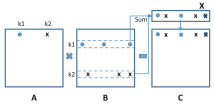
\includegraphics[width=.87\linewidth,keepaspectratio]{gustavsonRigheGraphicalIntel.svg.pdf}
	
\end{columns}
\blfootnote{Fred G. Gustavson «Two Fast Algorithms for Sparse Matrices: Multiplication and Permuted Transposition» 1978}
%Ri-adattamento estremamente compatto pseudocodice di algo gustvson SERIALE (3.4), originariamente basato su un accumulatore denso, 
%switch array per evitare acc. resets
%Paper molto citato, tra I primi contributi nell'ambito della moltiplicazione tra matrici SPARSE

\end{frame}

\begin{frame} {Formulazioni multi dimensionali}
\begin{columns}
	\column{0.70\textwidth}
	\begin{itemize}
		\item	ogni moltiplicazione di elementi non zero $a_{ik} \ast b_{kj}$\\
				(min. operazione assegnabile) è rappresentabile con voxel W(i,j,k)
		\pause
		\item	sottoinsiemi di W ottenuti fissando uno o due indici
		\begin{itemize}
			\item	Layers: W(i,:,:),W(:,j,:),W(:,:,k)
			\begin{itemize}
				\item	Partizionamento 1D
			\end{itemize}
		\end{itemize}
		\begin{itemize}
			\item	Fibers: Intersezioni di Layers relativi a indici diversi, e.g. W(i,j,:)
			\begin{itemize}
				\item	Partizionamento 2D
			\end{itemize}
		\end{itemize}
		\begin{itemize}
			\item	Cuboid: Sottoinsiemi di W 	
			\begin{itemize}
				\item	Partizionamento 3D
			\end{itemize}
		\end{itemize}
	\end{itemize}
	\column{0.30\textwidth}
	\includegraphics[width=.87\linewidth,keepaspectratio]{MM_cube.svg.pdf}
	\voidLine
	\includegraphics[width=.77\linewidth,keepaspectratio]{workCube3D.svg.pdf}
		
\end{columns}

%(Vari paper citano) Rappresentazione op: SpMM in un cubo di lavoro W , faccie A,B->C
%suddivisione lavoro in partizioni cubo
\end{frame}

\begin{frame} {Partitioned SpGEMM}
\begin{columns}
	\column{0.70\textwidth}
	\begin{itemize}
		\item	Partizionamento 2D del calcolo di C
		\begin{itemize}
			\item	Blocchi di C associati a gruppi di righe di A e colonne di B
		\end{itemize}
		\pause
		\item	Tradeoff tra:
		\begin{itemize}
			\item	overhead associato al partizionamento B 
			\item	Beneficio: |accumulatore denso| < |cache L2|
		\end{itemize}
	\end{itemize}
	\column{0.30\textwidth}
	\includegraphics[width=.87\linewidth,keepaspectratio]{gustavsonRigheBlocksGraphicalIntel.svg.pdf}
\end{columns}
\blfootnote{Patwary, M.M.A. et al. (2015) «Parallel Efficient Sparse Matrix-Matrix Multiplication on Multicore Platforms»}
%Sulla quale mi sono un pò più ispirato, ottimi risultati misurati rispetto a varie lib di alg.sparsa disponibili tra cui intel MKL
%BENEFICIO: accDenso fittato in cache(L2) -> durante le accumulazioni evito di andare a richiamare (CONTINUAMENTE) reg. Di memoria da strati cache inferiori (LLC/RAM)
%Overhead B: partizionamento in CSR separate + hyperSparsità => overhead di mem bandwidth … non molto chiaro
%Euristica sul vantaggio d'uso partizi
%e\_nnz = \frac{\sum\limits_{i:e\_nnz(i) > L2\_FP\_WORDS} e\_nnz(i)}
%{\sum\limits_{i=1}^m e\_nnz(i)} ~>~0.3
\end{frame}

\section{Fase simbolica:\\Determinazione dimensione del risultato}

\begin{frame}[fragile] {Fase simbolica di SpMM}
\begin{itemize}
	\item	Determinazione della dimensione (di porzioni) del prodotto
	\pause
	\item	Necessaria per evitare allocazioni dinamiche durante l'esecuzione parallela
	\begin{itemize}
		\item	e.g. non in linea con la filosofia OpenMP (e.g. \verb|#pragma omp cancel| default off)
	\end{itemize}
	\pause
	\voidLine
	\item	UpperBound nel caso row-by-row (formulazione $c_{i*} = \sum\limits_{k \in I_i(A)}  a_{ik} \ast  b_{k*}$):\\
	$| I_i(C) |~\leq~\sum\limits_{ j \in I_i(A) }  | I_j(B)  |$
	\begin{itemize}
		\item	Basso costo computazionale
		\item	Necessità di salvare i risultati intermedi in uno spazio temporaneo
	\end{itemize}
	\pause
	\item	Calcolo accurato
	\begin{itemize}
		\item	Maggior costo computazionale
		%\item	Determinazione esatta 
		\item	Salvataggio degl'indici degli elementi non zero di C\\
				senza eseguire le operazioni floating-point
		\item	Risultati intermedi direttamente nella matrice risultante
	\end{itemize}
\end{itemize}
%Focus su necessità di dare ad ogni thread conoscenza dove scrivere il blocco di risultati assegnato CONCORRENTEMENTE
\end{frame}

\begin{frame}[fragile] {UpperBound: Gestione dello spazio temporaneo}
\begin{itemize}
	\item	pre-partizionamento
	\item	Assegnazione dinamica
	\begin{itemize}
		\item	\begin{lstlisting}[basicstyle=\tiny,numbers=none]
sparsifyStartV = *@\bfseries \_\_atomic\_fetch\_add@*((acc->lastAssigned),nnz,__ATOMIC_ACQ_REL)
		\end{lstlisting}
		%alternativa con Verbatim
		%\begin{Verbatim}[commandchars=\\\{\}]
		%sparsifyStartV = \verbBoldize{__atomic_fetch_add}((acc->lastAssigned),nnz,__ATOMIC_ACQ_REL)
		%\end{Verbatim}

		\item	\begin{lstlisting}[basicstyle=\tiny,numbers=none]
*@\bfseries \#pragma omp atomic capture@*
{ 
sparsifyStartV = acc->lastAssigned;
acc->lastAssigned += nnz;
}
		\end{lstlisting}
		\item In entrambi i casi viene usata:   \verb|lock xadd|
	\end{itemize}
\end{itemize}
%Pre-partizionamento può richiedere formulazione UB ad hoc:
%caso 2D limitare formula precedente a partizioni di colonne... caso triplo prodotto diretto può essere più complicato
%a livello di cache consistency nessun problema grande -> zone di memoria soggette a cacheLines intersecate vengono accedute probabilmente in ordine diverso dai threads...
%
%dynAssign: NO LOCK (omp critical) --> NO FENCE 
%RMW -> atomicamente incremento indice ultimo elem.assegnato ritornando val precedente all'op
%                    (no risultati intermedi visibili tra I thread)
%:::APPROCCI EQUIVALENTI:::
%Lock prefix: consente al processore corrente di avere uso esclusivo di ogni memoria condivisa
%XADD tra nnz,lastIdx -> sparsifyStartV
%
%    accSparseStartIdx = __atomic_fetch_add(&(acc->lastAssigned),nnz,__ATOMIC_SEQ_CST); 
%    3ad2:       48 8b 45 e8             mov    -0x18(%rbp),%rax
%    3ad6:       48 83 c0 18             add    $0x18,%rax
%    3ada:       8b 55 f8                mov    -0x8(%rbp),%edx
%    3add:       f0 0f c1 10             lock xadd %edx,(%rax)
%    3ae1:       89 55 f4                mov    %edx,-0xc(%rbp)
\end{frame}

\begin{frame} {Determinazione accurata}
Percorrendo le operazioni effettuate nella formulazione row-by-row	
($c_{i*} = \sum\limits_{k \in I_i(A)}  a_{ik} \ast  b_{k*}$)
\begin{itemize}
	\item	Si inseriscono gli indici relativi alla matrice B \\
	come chiavi in una struttura indicizzata
	\pause
	\item	Porting in Userspace dei RedBlack Tree linux dal kernel 5.10.85 (LTS)
	\pause
	\item	Uso di un array di bitmaps
	\begin{itemize}
		\item	associando ad ogni indice uno specifico bit
		\item	Analogia con limb di una variabile a precisione arbitraria in GMP
	\end{itemize}
\end{itemize}
%Bitmaps implementati come array di flag generico (uchar array)  ---> similmente in paper originale gustavson
%O array di bitmaps
\end{frame}

%%%%% MULTI VERSIONING %%%%
%\begin{frame}[fragile] {Generazioni di versioni multiple di una funzione}
%\subtitle{Generazioni di versioni multiple di una funzione\\a tempo di pre-processamento}
%Obiettivi:
%\begin{itemize}
%	\item	Supportare efficientemente una doppia indicizzazione 
%	per l'integrazione in progetto fortran come 
%	\url{https://psctoolkit.github.io/products/amg4psblas/}
%	\pause
%	\item	Generazione efficiente di varie versioni del prodotto simbolico accurato per implementazioni
%	\begin{itemize}
%		\item	1D, 2D o triplo prodotto diretto
%	\end{itemize}
%\end{itemize}
%\pause
%\voidLine
%Meccanismo:
%\begin{itemize}
%	\item	Inclusione multiple dei sorgenti (generici)
%	\item	Ri-definizione di macro di configurazione usate nelle funzioni
%	\item	Modifica segnatura funzioni derivate mediante pre-processore
%\end{itemize}
%\voidLine
%\begin{lstlisting}[basicstyle=\tiny,numbers=none]
%spmat* CAT( spmmRowByRow_SymbNum_ , OFF_F )  ( spmat * A , spmat * B , CONFIG * cfg ){...} 
%\end{lstlisting}
%%%%%%%%%%%%%%%%%%%%%%%%%%%
%
%%Caso integrazione Fortran (processo di integrazione avviato) molto utile per evitare shifting iniziale complessivo, usato largamente nel codice 
%%Multi versioning in generale ( 8 VERSIONI DELLE FUNZIONI BASE):
%%Evito uso massiccio di condizioni nel codice (cmq gestiti benissimo da predittori) 
%%Esclusione blocchi di codice non necessari 
%%  --> maggiore ottimizzabilità in compilazione 
%%Segnature diverse da CAT: operatore pre-processore ## wrappato (concat preprocessor token ESPANSI) 
%\end{frame}

\section{Fase numerica: calcolo del prodotto tra matrici}

\begin{frame}[fragile]  {Implementazioni 2D}
\begin{columns}
	\column{0.55\textwidth}
	\begin{itemize}
		\item	blocchi di righe e colonne ai thread (3-5)
		\item	Moltiplicazioni scalari (16) tra
		\begin{itemize}
			\item	$a_{ij}$
			\item	righe $b_{j*}$ della partizione di B assegnata
			\item	uso accumulatore denso
		\end{itemize}
		\item	partizionamento colonne della matrice B\\
				\emph{inplace} o in sotto-matrici dedicate
		\item	"Sparsificazione" (20-24)
	\end{itemize}

	\column{0.45\textwidth}
	\begin{lstlisting}
#pragma omp parallel for schedule(runtime) private(accV,...)
for (tileID = 0; tileID < gridSize; tileID++){
  t_i = tileID/cfg->gridCols;  //i-th row block
  t_j = tileID%cfg->gridCols;  //j-th col block
  colPart = colPartsB + t_j;
  accV = accVectors + tileID; 
  for (ulong r=startRow;  r<startRow+rowBlock;  r++){
    //row-by-row restricted for AB[r][:colBlock:]
    for (ulong j=A->IRP[r]-OFF_F,c,bRowStart,bRowLen; 
     j<A->IRP[r+1]-OFF_F; j++){

      c = A->JA[j]-OFF_F;
      bRowStart = colPart->IRP[c];
      bRowLen   = colPart->RL[c];
      CAT(scSparseVectMulPart_,OFF_F)(A->AS[j],
       colPart->AS+bRowStart,colPart->JA+bRowStart,...);
    }
    accRow = outAccumul->accs + IDX2D(r,t_j,cfg->gridCols);
    #if SPARSIFY_PRE_PARTITIONING == T
    _sparsifyUB(accV,accRow,startCol);
    #else
    sparsifyUBNoPartsBounds(outAccumul,accV,accRow,startCol);
    #endif
    _resetAccVect(accV);
  }
}
if (mergeRowsPartitions(outAccumul->accs,AB,cfg)) goto _err;
	\end{lstlisting}
\end{columns}
	\begin{figure}[H]
  	\centering
	\includegraphics[width=.25\linewidth,keepaspectratio]{gustavsonRigheBlocksGraphicalIntel.svg.pdf}
	\end{figure}
\end{frame}

\begin{frame}[fragile]  {Triplo prodotto Diretto}
\begin{columns}
	\column{0.55\textwidth}
	Calcolo $AC_{i+1} = R \cdot AC \cdot P$
	\begin{itemize}
		\item	Calcolata una riga di $R \cdot AC$\\
		in accumulatore denso (8)
		\item	"Forwardata" immediatamente per indicizzare P
		secondo la formulazione row-by-row (11-13)
		\item	"Sparsificazione" $R\cdot AC\cdot P$ (15)
		\item	Nessuna matrice intermedia prodotta
	\end{itemize}
\column{0.45\textwidth}
	\begin{lstlisting}
#pragma omp parallel for schedule(runtime) private(accRAC...)
for (ulong r=0;  r<R->M; r++){  //row-by-row formulation
  //iterate over nz entry index c inside current row r
  accRAC  = accVectorsR_AC  + omp_get_thread_num();
  accRACP = accVectorsRAC_P + omp_get_thread_num();
  //computing (tmp) R*AC r-th row
  for (idx_t j=R->IRP[r]-OFF_F; j<R->IRP[r+1]-OFF_F; j++)
    CAT(scSparseRowMul_,OFF_F)
     (R->AS[j], AC, R->JA[j]-OFF_F, accRAC);
  //forward the computed row
  for (idx_t j=0; j<accRAC->nnzIdxMap.len; j++){
    c = accRAC->nnzIdx[j];  
    CAT(scSparseRowMul_,OFF_F)(accRAC->v[c],P,c,accRACP);
  }
  sparsifyUBNoPartsBounds(outAccumul,accRACP,...);
  ...
  _resetAccVect(accRAC);
  _resetAccVect(accRACP);
}
if (mergeRows(outAccumul->accs,out))  goto _err;
	\end{lstlisting}
\end{columns}
\end{frame}

\section{Performance}
\begin{frame} {Classi di input utilizzati}
\begin{columns}
	\column{0.65\textwidth}
	Ambiente di test
	\begin{itemize}
		\item	OS: CentOS Stream 8
		\item	CPU: Intel Xeon Silver 4210 2.20 GHz 40 core
		\item	RAM: 64GB
	\end{itemize}
	\pause
	\voidLine
	sistema lineare ottenuto da 
	\pause
	\begin{itemize}
		\item	discretizzazione alle differenze finite PDE di 2° ordine\\
		griglia regolare e condizioni al contorno di Dirichlet
		\pause
		\item	generazione degli aggregati nei AMG
		\begin{itemize}
			\item	Matching
			\item	Vanek-Brezina
		\end{itemize}
		\item	Con e senza Smoothing
		\pause
		\item	Considerati valori medi di 40 ripetizioni
	\end{itemize}
	\column{0.35\textwidth}
	\tiny Matching Smoothed\quad\quad-\quad\quad Non Smoothed\\
	\includegraphics[width=\linewidth,keepaspectratio]{sparseMatrices/matchingMediumSmoothed_UnSmoothed.ppm.png}
	\voidLine
	\voidLine
	\tiny Vanek-Brezina Smoothed\quad-\quad Non Smoothed\\ 
	\includegraphics[width=\linewidth,keepaspectratio]{sparseMatrices/varnekBrenzina_MediumSmoothed_UnSmoothed.ppm.png}
\end{columns}
%Struttura diagonale tipica da config discretizzazione (esempio PARGEN in (amg4)psblas)
%Visualizzazione nnz mediante mapping:
%tile in matrice sparsa --> pixel (or-ing)
%È stato difficile eseguire I test senza sovrapposizioni con altri ... cercato di farlo con script light basato su top (nice 20)
\end{frame}

%\begin{frame}[fragile]  {OpenMP scheduling e chunksize}
%Data una parallelizzazione di un ciclo for:\\
%\begin{lstlisting}
%((CHUNKS_DISTR_INTERF) cfg->chunkDistrbFunc) (gridSize,AB,cfg);
%#pragma omp parallel for schedule(runtime) private(accV,...)
%for (tileID = 0; tileID < gridSize; tileID++){
%\end{lstlisting}
%\pause
%\begin{itemize}
%	\item	scheduling static
%	\begin{itemize}
%		\item	blocchi di iterazioni (\emph{chunksize}) "fair" \\
%		e.g. $\frac{nIter}{nThread}$ iterazioni per thread
%	\end{itemize}
%	\pause
%	\item	scheduling dynamic 
%	\begin{itemize}
%		\item	dimensione blocco di iterazioni = 1 di default
%		\item	possibilità ai thread di proseguire il calcolo\\
%				al termine del loro blocco di iterazioni
%		\begin{itemize}
%			\item	utile nel caso di costo per iterazione sbilanciato
%		\end{itemize}
%		\pause
%		\item	false cache sharing
%		\pause
%		\item	adattamento del chunksize:\\
%		$\frac{nIter}{nThread*K}$ iterazioni per thread
%	\end{itemize}
%\end{itemize}
%\end{frame}

\begin{frame}[fragile] {Configurazione}

{\bf Schedule Dynamic OpenMP}	\quad- assegnamento iterazioni
\begin{itemize}
	\item	chunksize: $\frac{it}{nThread*4}$
\end{itemize}
\voidLine
\pause
{\bf Griglia di partizionamento}	\quad- strutturazione iterazioni
\begin{itemize}
	\item Implementazioni 1D
	\begin{itemize}
		\item Suddivisione righe in nThread o 2*nThread blocchi
	\end{itemize}
	\item Implementazioni 2D
	\begin{itemize}
		\item Suddivisione calcolo di C in blocchi 2D
		da una griglia $gridRows \times gridCols$
		\item Porting \verb|MPI_Dims_create| da OpenMPI
		\begin{itemize}
			\item suddividendo nthread+1 per numeri primi
		\end{itemize}
	\end{itemize}
\end{itemize}
%Configurazione tenuta costante nei test per ridurre il numero di elementi variabili -> riducendo il numero di test da eseguire
%Griglia di partizionamento (suddivisione lavoro tra I thread) --> adattamento num thread configurato
%Caso 2D testato solo con MPI_Dims_create, altro non ho avuto possibilità dato server molto occupato
%MPI_Dims.. : #processori<-#thread, usata per determinare una topologia 
%Nel contesto della programmazione a memoria distribuita, la funzione
%MPI_Dims_create consente di determinare una suddivisone bilanciata di un numero
%di processi in una topologia cartesiana n-dimensionale da utilizzare durante il calcolo

\end{frame}

\begin{frame} {Migliore assegnamento spazio temporaneo}
%\begin{columns}
	%\column{.50\textwidth}
	%\begin{itemize}
	%	\item	guadagno nell'uso assegnamento dinamico per implementazioni 1D
	%	\item	prestazioni simili per implementazioni 2D
	%	\item	
	%\end{itemize}
	%\column{.50\textwidth}
	\centering
	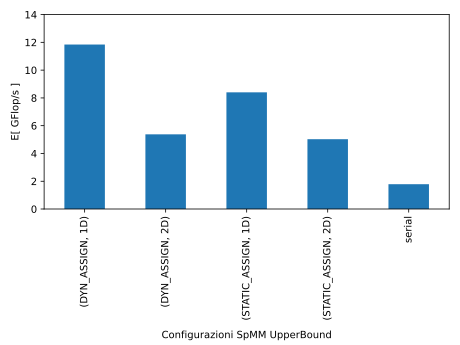
\includegraphics[width=.65\linewidth,keepaspectratio]{graphs/q1.svg.pdf}
%\end{columns}
%Valori medi su tutti le impl. SpMM UB, con le configurazioni indicate...
%Assegnamento dinamico da un vantaggio in implementazioni 1D, non significativo in implementazioni 2D
%in generale si assegnano ai thread blocchi di righe medio/grandi 
%False Cache Sharing Note:
%interferenze ai bordi dello spazio di "sparsificazione" ridotto/assente dato che:
%    Tempo thread a raggiunge la fine in collisione col thread B, il thread B è già andato avanti
%
%volendo con questo si può giustificare un extra costo in assign statico per overhead partizionamento spazio allocato
\end{frame}
\begin{frame} {Migliore dimensione di bitmap}
	\centering
	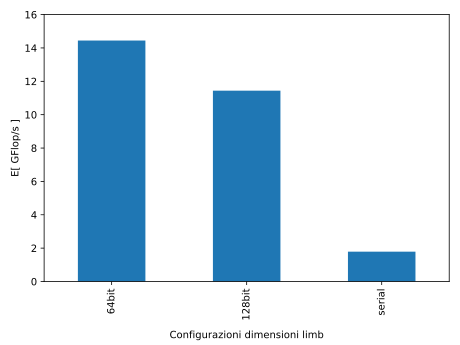
\includegraphics[width=.65\linewidth,keepaspectratio]{graphs/q2.svg.pdf}
%Valori medi su tutte le implementazioni SpMM IDXMAP, con config indicate
\end{frame}

\begin{frame} {Migliore implementazione per classe di input}
\begin{columns}
	\column{.50\textwidth}
	Implementazione/configurazione migliore\\
	variabile in base alla classe di input
	\pause
	\begin{itemize}
		\item	Triplo prodotto tendenzialmente meglio
		\pause
		\item	Maggiore efficienza implementazioni\\
		su classi di input Smoothed
		\pause
		\item	UpperBound: 1D migliore di 2D\\
		in classi Smoothed, 
		\item	viceversa per le classi Unsmoothed
	\end{itemize}
	
	\column{.5\textwidth}
	\includegraphics[width=\linewidth,keepaspectratio]{graphs/q3.svg.pdf}
\end{columns}
%Valori medi su tutte le run, con configurazion indicate
\end{frame}

\begin{frame} {Confronto con implementazione seriale}
\begin{columns}
	\column{.5\textwidth}
	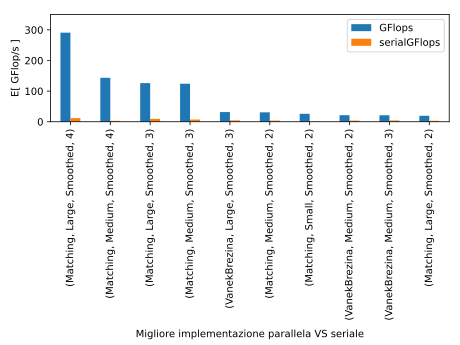
\includegraphics[width=.87\linewidth,keepaspectratio]{graphs/q4-b.svg.pdf}
	\column{.5\textwidth}
	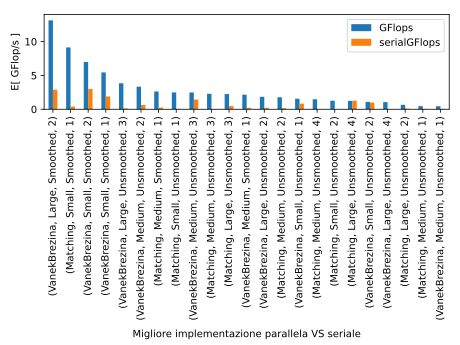
\includegraphics[width=.87\linewidth,keepaspectratio]{graphs/q4-s.svg.pdf}
\end{columns}
%Confronto implementazione/configurazione migliore per ogni matrice...
%Visibile come implementazioni seriali sono (quasi) sempre abbastanza peggio
\end{frame}
\begin{frame} {Numero thread variabile}
	\centering
	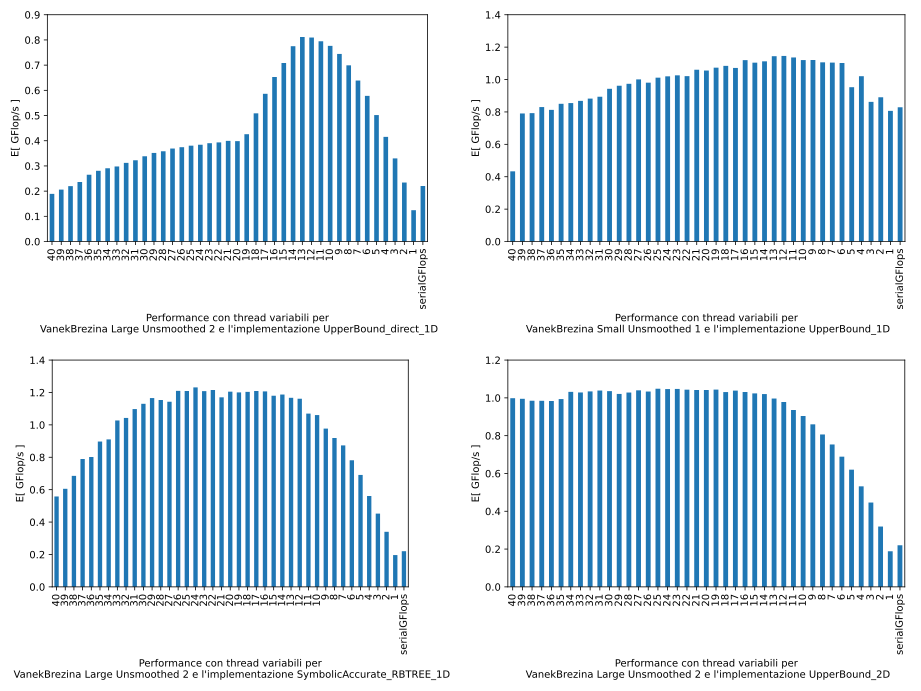
\includegraphics[width=.68\linewidth,keepaspectratio]{graphs/q5.svg.pdf}
\end{frame}
\begin{frame} {Conclusioni}
\begin{itemize}
	\item	Pattern di sparsità dei non zeri degli input 
	determina uno sbilanciamento nel carico di lavoro assegnato
	dipendente da:
	\pause
	\begin{itemize}
		\item	L'approccio di divisione del lavoro usato
		\item	Tipologia di implementazione
		\item	Livello di concorrenza
	\end{itemize}
	\pause
	\item	Lo scheduling di un alto numero di thread può essere sconveniente
	\begin{itemize}
		\item	Overhead init-scheduling openMP visibile in config. mono thread
	\end{itemize}
	\pause
\end{itemize}
\voidLine
%Sviluppi futuri
%\pause
%\begin{itemize}
%	\item	Analisi dettagliata sul livello di parallelismo ottimale per classe di input
%	\pause
%	\item	Estensione implementazioni
%	\pause
%	\item	Implementazione formulazioni ESC Outer-Product
%	\pause
%\end{itemize}
\end{frame}

%%%%%%%%%%%%%%%%%%%%%%  RISERVE  %%%%%%%%%%%%%%%%%%%%%%%%%%%%%%%%%%%%%%%%%%%%%%%
\appendix
\backupbegin


\begin{frame} {Contesto Applicativo}%{Contesto del Problema affrontato}
\begin{columns}
	\column{0.78\textwidth}
	\begin{itemize}
		\item	Soluzioni di {\bf P}artial {\bf D}ifferential {\bf E}quation (PDE) mediante\\
		tecniche numeriche per risoluzioni all'interno di dominii 2D o 3D
		\begin{itemize}
			\item	Griglie di discretizzazioni per 
			approssimare derivate in differenze nei punti di una mesh
		\end{itemize}
		\pause
		\item	Derivazione di Sistemi Lineari
		\pause
		\begin{itemize}
			\item	{\bf Sparsi}, per la maggior parte delle tecniche numeriche:
			\begin{itemize}
				\item differenze finite
				\item	elementi finiti
				\item	volumi finiti
			\end{itemize}
		\end{itemize}
	\end{itemize}
	\column{0.22\textwidth}
	\includegraphics[width=.87\linewidth,keepaspectratio]{5PointStencil.png}
	
\end{columns}
\blfootnote{Valeria Cardellini Davide Barbieri Alessandro Fanfarillo Salvatore Filippone   
	«Sparse Matrix-Vector Multiplication on GPGPUs»\\
	R. J. LeVeque. «Finite Difference Methods for Ordinary and Partial Differential Equations»\\
	A. Quarteroni e A. Valli. «Numerical Approximation of Partial Differential Equations»\\
	S. V. Patankar. «Numerical Heat Transfer and Fluid Flow»
}
%Una delle possibili origini di Sistemi lineari sparsi: Numerical PDE solve (A dx stencil a 5 punti)
%Diversi studi evidenziano la sparsità dei sysLin generati, dato che:
%il numero di elementi in ogni equazione discretizzata dipende da proprietà topologiche locali alla discretizzazione 
%e non dalla dimensione globale del dominio del problema da risolvere

\end{frame}

\begin{frame} {Importanza della sparsità della matrice}
\subtitle{solutori iterativi vs diretti}
\begin{columns}
	\column{0.77\textwidth}
	\begin{itemize}
		\item	Solutori {\bf iterativi} generano una serie di \underline{soluzioni intermedie}\\
		(ipoteticamente) convergenti alla soluzione del sistema $x^{\ast}$
		\begin{itemize}
			\item	\underline{Mantenendo le proprietà di sparsità} di A nei risultati intermedi
		\end{itemize}
		\pause
		\item	Solutori {\bf diretti} trovano la soluzione del sistema x* impiegando 
		una \underline{fattorizzazione della matrice A} in matrici di struttura semplice 
		\begin{itemize}
			\item	Spesso \underline{perdendo le proprietà di sparsità} della matrice
		\end{itemize}
	\end{itemize}
	\column{0.23\textwidth}
	\includegraphics[width=.87\linewidth,keepaspectratio]{Efficient_Linear_System_Solvers_for_Mesh_Processing_densificationByDirectSolverSimplied.svg.png}
\end{columns}
\blfootnote{David Bommes Mario Botsch e Leif Kobbelt. «Efficient Linear System Solvers for Mesh Processing»}
%Perdità sparsità + problema border line capacità computaz. (NNZ ragionevole MA dim matrice enorme)
% ==> compute overhead, unfit in mem
%Esempio a destra, fattorizzazione di una matrice 500x500 con soli 3502 elementi
%36000 non zero con il metodo di Cholesky in alto a sinistra
%14000 non zero con il metodo di Cuthill-McKee in alto a destra
%6203 non zero con il metodo minimum degree ordering in basso a destra
%7142 non zero con il metodo nested dissection method in basso a sinistra
\end{frame}

\begin{frame}<presentation:0>[noframenumbering] {Solutori iterativi basati su metodi MultiGrid}
\begin{columns}
	\column{0.64\textwidth}
	\begin{itemize}
		\item	Usando un metodo iterativo basico\\
		si applicano delle correzioni ai residui 
		\pause
		\item	Risolvendo un \underline{sotto problema} dell’originale \\
		con un \underline{sottoinsieme delle incognite}
		\item	Ricorsivamente, fin quando conveniente\\
	\end{itemize}
	\pause
	\column{0.36\textwidth}
	\includegraphics[width=.87\linewidth,keepaspectratio]{Multigrid_Visualization_wikipedia.png}
\end{columns}
\begin{itemize}
	\item	{\bf Geometric MG vs Algebric MG}
	\begin{itemize}
		\item	AMG richiedono unicamente la matrice A per generare i sotto problemi
		%\begin{itemize}
		%	\item	\underline{Usando ripetutamente il {\bf prodotto di Galerkin} nella fase di setup}
		%\end{itemize}
		\item	Applicabili alla risoluzione di \underline{problemi discretizzati con griglie non strutturate}
	\end{itemize}
	\pause
	\item	{\bf Scalabilità}
	\begin{itemize}
		\item	numero di iterazioni e costo per iterazione\\
		circa costante all’incrementare della dimensione
	\end{itemize}
\end{itemize}
%correzioni alle soluzioni approssimate ottenute con un metodo iterativo basico.
%applicate ai residui associati agli errori delle soluzioni intermedie
%risolvendo un sotto problema dell’originale contente un sottoinsieme delle incognite.
%
%Il sotto problema può essere risolto a sua volta applicando ricorsivamente delle
%correzioni a dei sotto problemi ulteriori, 
%sempre più piccoli e facili da risolvere, fino
%a quando la risoluzione dell’ultimo sotto problema è di una difficoltà trascurabile
%rispetto a generarne un altro.
%
%Le iterazioni di questi metodi possono essere strutturati con cicli di varia natura.
%Tra le metodologie principalmente utilizzati ci sono cicli a forma V, F e W.
\end{frame}


\begin{frame}{Formulazione Outer Product}
\subtitle{Expand Sort Compress – propagation blocking}
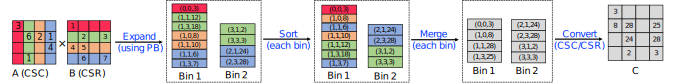
\includegraphics[width=.87\linewidth,keepaspectratio]{OuterProduct_PBAlgoritmExample_ESC.svg.pdf}
\begin{columns}
	\column{0.8\textwidth}
	\begin{itemize}
		%\item	Approccio Expand – Sort – Merge
		\item	Prodotti eseguiti in parallelo nella fase di expand
		\item	risultati in formato COO, raggruppati in bin {\tiny( \emph{lazy} propagation blocking)}
		\pause
		\item	Riduzione dei risultati intermedi mediante sort e merge (add)
		\pause
		\item	Migliore utilizzo della memoria rispetto a row-by-row e col-by-col
		%\begin{itemize}
		%	\item	accesso randomico (dal pattern di sparsità dei non zeri) 
		%	alle righe/colonne di una delle matrici
		%\end{itemize}
	\end{itemize}
	\column{0.2\textwidth}
	\includegraphics[width=.87\linewidth,keepaspectratio]{OuterProduct_PBAlgo_BinsExample_ESC.svg.pdf}
\end{columns}
\blfootnote{David Edelsohn Ariful Azad Zhixiang Gu Jose Moreira\\
«Bandwidth Optimized Parallel Algorithms for Sparse Matrix-Matrix Multiplication using Propagation Blocking»}
%Outer product effettuato in parallelo ( coppie row-col per thread)
%aggregazione derivata da riga di in A  in bin locali (flush periodici da bin locali ai thread)
%riduzione con sort -> add entry con stesse coordinate
\end{frame}

\begin{frame} {Implementazioni Multi Dimensionali}
\begin{columns}
	\column{0.5\textwidth}
	\centering
	SparseSUMMA 
	\begin{figure}[H]
  	\centering
	\includegraphics[width=.67\linewidth,keepaspectratio]{sparseSUMMAIteration.png}
	\end{figure}

	\column{0.5\textwidth}
	\centering
	Split3DSpMM
	\begin{figure}[H]
  	\centering
	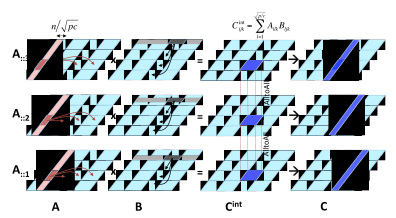
\includegraphics[width=.67\linewidth,keepaspectratio]{Split3DSpMMIteration.png}
	\end{figure}
\end{columns}
\blfootnote{Buluç, Aydin \& Gilbert, John. (2011).
«Parallel Sparse Matrix-Matrix Multiplication and Indexing: Implementation and Experiments»\\
Azad, Ariful \& Ballard, Grey \& Buluç, Aydin \& Demmel, James \& Grigori, Laura \& Schwartz, Oded \& Toledo, Sivan \& Williams, Samuel. (2015). 
«Exploiting Multiple Levels of Parallelism in Sparse Matrix-Matrix Multiplication»
}
%2 algoritmi, pensati per sys a DISTRI-MEM, con partizionamento 2D e 3D, Ordinatamente:
%sparseSUMMA (sparsificazione controparte alg.denso) uso di outer product per moltiplicazione partizioni relative A<->B(in DCSC <- ipersparsità blocchi di mat.sparsa), 
%accumulando I blocchi con inner-product (std formul) nel blocco finale in C
%VERSIONE 3D, partizionamento ulteriore blocchi di A in una mesh logica di processi 3D
\end{frame}
\backupend


\end{document}

%buid template
%~/DATA/SW/latex/2021/bin/x86_64-linux/pdflatex -jobname=out -output-directory=/tmp/p presentazione.tex
